%%%%%%%%%%%%%%%%%%%%%%%%%%%%%%%%%%
% EL/EEE Report Template
% University of Southampton
%
% authors: Ben Rowlinson
%          Lawrence Gray 
%          Joel Trickey
%          Joseph Hindmarsh
%          Mohammed Ibrahim
%
% edited : 2017-03-16
%%%%%%%%%%%%%%%%%%%%%%%%%%%%%%%%%%

\documentclass[a4paper,11pt]{article}

%%%%%%%%%%%%%%%%%%%%%%%%%%%%%%%%%%
% PACKAGES
%%%%%%%%%%%%%%%%%%%%%%%%%%%%%%%%%%
\usepackage[margin=1in]{geometry}
\usepackage{amsmath}
\usepackage{graphicx}
\usepackage{wrapfig}
\usepackage{microtype}
\usepackage[T1]{fontenc}
\usepackage{array}
\usepackage[utf8]{inputenc}
\usepackage[margin=1in]{geometry}
\usepackage{caption} % for sub-figure
\usepackage{subcaption}% for sub-figure
\renewcommand{\baselinestretch}{1.2} % line spacing

%%%%%%%%%%%%%%%%%%%%%%%%%%%%%%%%%%
% DOCUMENT BEGIN
%%%%%%%%%%%%%%%%%%%%%%%%%%%%%%%%%%
\begin{document}
  
\begin{center}
{\Large{\textbf{ELEC2205 D4 -- Systems Design Exercise}}} \\ [\baselineskip]
Team Ganges \\
Ben Rowlinson, Lawrence Gray, Joel Trickey,\\ Joseph Hindmarsh and Mohammed Ibrahim\\
17 March 2017\\
\end{center}

\tableofcontents
\newpage

\listoffigures
\newpage

\section{Challenge Solution Statement}
\subsection{Challenges}
Same-day parcel delivery is a difficult proposition for many businesses, even those that restrict the service to large cities. The current solution of couriers using vans and motorcycles is inefficient due to congestion in built up areas, especially if the deliveries are spread out across a delivery district. To improve efficiency of small parcel deliveries, Team Ganges proudly presents its Project Itchen prototype – a UAV designed from the ground up for cargo transport. By opening the skies to Itchen for its deliveries, same-day delivery will no longer be restricted to cities and become a reality for customers across the country.\\ 
Many commercially available UAVs exist on the market already, however the key thing holding them back from adoption in the deliveries market is the question of cargo. The most common type of payload-carrying drone is a camera drone, which has the payload securely affixed to the drone chassis. This is excellent during flight, but is less optimal for package delivery, as the recipient would have to approach the live UAV to remove the package. To solve this challenge, Team Ganges will provide a mechanism to drop-off the package once it has reached its destination and is at a low enough altitude. This will reduce the turn-around time of the drone and allow it to drop-off the package when the recipient is not present.\\
The solution concept also addresses the problem of interference with other transmitters, through avoiding the use of a commercial transmitter in favour of a proprietary solution. This allows for the communications between the UAV and the Base Station to be encrypted, and the UAV identify true instructions from the base station over interference from other users and devices.\\
\newpage
\subsection{Specification}
\begin{itemize}
\item The UAV should use 4 2205 2300kV motors
\item The motors must use an arming procedure
\item The propellers shall be 5" in diameter with a pitch of 3"/rev
\item Motor speeds shall be controlled by 1-2ms PWM ESCs (Electronic Speed Controllers)
\item The UAV shall be powered by a single 3 Cell LiPo battery
\item The battery capacity should be more than 1500mAh
\item The Communications shall be in the ISM radio frequency band
\item Telemetry data could be transmitted back to the base station
\item Telemetry data could be stored locally on an SD Card 
\item Telemetry Transmission rate should be 1 packet/second
\item The IMU should produce new data at least 100 times per second
\item The UAV should be able to drop off cargo whilst in flight
\item The UAV could be able to pick up cargo whilst in flight
\item The communications could be encrypted
\item Packet loss from the communications should be less than 1 in 100
\item Communications speed should be at least 400 packets/second (One 10-bit word per packet)
\item The PID gain constants could be updated over the communications uplink
\item The UAV should be able to detect altitudes of between 15cm to 100cm
\item The control loop should update at a rate of at least 100 times/second to match IMU 
\item The UAV should warn the user of low battery status
\item The chassis should have a centre of mass within 5cm of the geometric centre
\item UAV should recover from a 15 degree inclination
\end{itemize}

\newpage
\section{System Design}
\subsection{High Level Block Diagram}
Appendix C gives a high-level block diagram of the final design of the system.
\subsection{UAV}
On-board the drone, there are two micro-controllers - an Arduino Leonardo and an Il Matto.\\
The Leonardo handles the PID control to ensure stable flight according to the user's control inputs. It achieves this by receiving angle data from a IMU module over an I2C interface and controller inputs from the Il Matto using UART. After processing this data, it controls the flight of the UAV through four PWM channels to four ESCs, which in turn control four 2205 brushless motors using 3-phase AC power.\\
The Il Matto is responsible for receiving the user's inputs from the transceiver module and passing on potentiometer data to the Leonardo when requested. It also controls a servo using PWM to raise and lower the cargo hook as per the data received from switches on the ground. It also sends telemetry received from an IR sensor and a battery voltage circuit back to the ground through the transceivers. SD card is not present on the final design.\\
This system is powered by a 1550mAh 11.1V LiPo battery via a power distribution circuit that ensures the correct voltage is supplied to each component on-board the UAV.\\
For the chassis, a clear acrylic I-frame was laser-cut and glued together with Super Glue.\\
Using two micro-controllers to handle control and communications separately, allows the control to remain accurate by reducing computational strain, and a faster data rate from the ground to be achieved. The PWM outputs to the ESCs only use a very small range of timer values. This requires the timers to have a high precision to ensure fine control of the motors. Initially, an Il Matto was considered for the control but as this only supplies one 16-bit timer and two 8-bit timers, it was decided that this would not supply the required precision. The Leonardo on the other hand has two 16-bit timers with 4 outputs which allow sufficient control of its PWM outputs.\\
For communications, the Il Matto was used as we have experience of programming it, and it has the required hardware to interface with the various modules on the drone.\\
\subsection{Communications}
The ground control and the drone communicate with each other over a 433MHz FSK scheme using RFM12B-S2 transceiver modules. These modules are both controlled by Il Mattos using the SPI protocol and a micro-controller library. Potentiometer and switch data is sent to the drone and telemetry is sent back to the base.\\
The Spektrum DX6e remote control transmitter and receiver system was rejected at the design stage as it would require taking four PWM outputs from the receiver into the micro-controller which proved difficult in early testing.\\ 
\subsection{Ground Control}
On the ground, an Il Matto uses its built-in ADC to take four different analogue voltages from two X-Y potentiometers for user-controlled thrust, yaw, pitch, and roll. It sends this data to a transceiver for transmission to the drone. Switches taken as inputs to the Il-Matto, allow the user to control the cargo hook, toggle between PID and flight mode, and activate a kill switch for safety. A UART interface with a PC allows telemetry to be read and logged, and new K values for the PID controller to be input.\\
As an Il Matto was being used with the transceiver on the drone, the use of an Il Matto on the ground made software easier to develop.\\

\section{Design Evaluation}
\subsection{Difficulty of Specification Attempted}
At the start of this project we knew we wanted to choose a design which was challenging, but also achievable.
We knew early on that we didn't want to accept the pre-built controller and instead build our own proprietary one. This helped us to achieve practical two-way communications between ground and air. 
We wanted to devolve as much of the responsibility for control from the pilot by using absolute angle measurements to provide feedback to the UAV. This poses a more difficult control problem and although we have a demonstrably working control system, we were not able to achieve full, independent, stable flight.
Designing and building our own chassis out of acrylic sheets allowed us to come in on budget, but meant that the frame was extremely brittle and heavy, meaning testing the drone safely and non-destructively became a challenge.
Our successful extra features; servo-actuated cargo acquisition, IR sensor telemetry, real-time PID tuning, communications encryption, battery voltage reading were only integrated once the more critical modules had been completed. 
\subsection{Quality of Electronic Design}
We wanted separate micro-controllers for the on-board communications and control modules. This presented the considerable problem of synchronising communications between these two sub-systems. 
Utilising the on-chip DMP on the IMU allowed us to acquire pre-processed attitude data which massively reduced the computing strain on our micro-controller. This gives us parallel processing of the past and present IMU data thus giving us a finer resolution for control. This introduces the problem of synchronising these separate processes. 
Use of PWM controlled ESCs meant we needed 4 16-bit timer outputs from the control sub-system to finely adjust our motors. This meant upgrading to a more powerful micro-controller.
The Power Distribution Board (PDB) meant we could power all the on-board components from the same supply and meant we could reliably power up. This did increase the weight of the drone.
\subsection{Ease of Use}
Our start-up sequence includes a number of safety features; IMU settling time, motor arming sequence, optional ESC calibration. 
The pilot interface is a standard UAV set-up, except that the throttle is centred at zero and not free-floating. 
The controller is ergonomic and can be run off batteries. 
The current lack of LEDs indicating the front makes piloting difficult at large distances.
\subsection{Creativity and Innovation}
We designed our own servo-actuated cargo hook to enable quick and easy pick-up and drop-off of the cargo. This adds weight and complexity to the electronics, but was easy to bolt onto the critical path design.
We were able to read the altitude and battery level in real time using a serial terminal. This could be implemented using the Il Matto TFT screen so the Laptop isn't required.
The ability to repair the chassis quickly and easily allowed for rapid testing, but this unbalanced the weight distribution of the drone and led to inconsistent test flights.
\subsection{Aesthetics}
Transparent acrylic chassis is less of an eye-sore, but equally makes piloting at a long distance difficult. Etching into the plastic to add our company name makes it easily identifiable as a brand.
Our controller also matches the aesthetic style of the drone. The switches are placed at convenient locations for rapid killing of motors if necessary.
The coat-hanger wire propeller guards are minimalistic but robust enough to deal with low velocity impacts.
As this is still a prototype there are flying wires used but we used ribbon cable wherever possible to minimise crossed wires.
\subsection{Cost}
\#\#\#DO SOMETHING HERE\#\#\#
\subsection{Reliability}
The UAV powers up correctly and consistently on connection to the LiPo.
The Communications system was heavily tested to ensure we could conduct test flights safely.
We achieved tethered single axis stability through a number of tests.
The current cargo acquisition hook doesn't fully extend and gets stuck in a particular position.
We cannot reliably achieve stable flight, but this only requires tuning of the PID gains.
Throughout our fully integrated testing, the electronics systems remained robust and very rarely experienced a failure.
The chassis performed very well with regard to protecting the electronics from impacts.

\section{Costing, Marketing and Conformance Marking}
\subsection{Costing}
In the project proposal form, estimates were made towards the costings. Now that the project is done, more realistic estimates can be made. This cost differs from this original as more components were included in the project than originally planned and some components broke in the testing process so the prices in Table 1 includes replacements for those parts.
\begin{table}[htp]
\begin{tabular}{|l|l|l|l|}
	\hline
	Component & Amount & Single Cost/\textsterling & Bulk Cost/\textsterling  \\
	\hline
	20A ESC & 4 & 23.95 & 23.95\\
	\hline
	Clockwise 2204 2300KV motors & 2 & 11.78 & 11.78\\
	\hline
    Counter-Clockwise 2204 2300KV motors & 2 & 11.78 & 11.78\\
	\hline
    Thumb Joystick & 2 & 10.39 & 3.98\\
	\hline
	Propeller Pack & 1 & 1.25 & 1.00\\
	\hline
	Female XT60 battery connector & 1 & 1.00 & 1.00\\
	\hline
	ESC Connector Pack & 1 & 3.50 & 1.99\\
	\hline
	1550MAh LiPo Battery & 1 & 14.99 & 12.86\\
	\hline    
	Arduino Leonardo & 1 & 18.50 & 5.64\\
	\hline
	RFM12B-S2 transceiver modules & 2 & 12.00 & 3.78\\
	\hline
	5V Regulator & 1 & 1.63 & 0.79\\
	\hline
	LiPo Charger & 1 & 14.99 & 14.99\\
	\hline
	Atmel At-Mega 644p & 2 & 12.62 & 7.24 \\ 
	\hline
	Micro Servo & 1 & 7.70 & 1.93\\ 
	\hline
	MPU-6050 Gyroscope Chip & 1 & 1.50 & 1.50 \\ 
	\hline
	Miscellaneous  & 1 & 8.00 & 6.00\\ 
	\hline
	A2 5mm acrylic sheet  & 2 & 21.10 & 8.49 \\ 
	\hline
	A4 3mm acrylic sheet  & 1 & 2.64 & 1.35\\ 
	\hline
    Labour (\textsterling20/hour)  & 2 & 0 & 40\\ 
	\hline
	\textbf{Total}& &179.32&160.05\\
	\hline
\end{tabular}
\caption{Table showing total costings for parts for prototyping and manufacturing}
\end{table}
\subsection{Manufacturing Costs}
The bulk cost includes the labour costing for manufacturing the quad-copter. This was estimated to be 2 hours. The two hours broken down are as follows; A skilled worker will first laser cut the frame and glue it together which should take 30 minutes. They then must program all of the micro-controllers and calibrate the ESCs, this should take another 10 minutes. The circuits should take 40 minutes to connect together and mount. Finally, the last 40 minutes will be spent on testing and verifying that everything is in a working order.\\
\subsection{Person-Hours}
There are other costs that also need to be considered, the first being person-hours for the development. From the time sheet that we filled out throughout the project there was an estimated 700 hours that was spent on developing and building the quad-copter. At \textsterling75 an hour this comes to \textsterling52,500. This time can be split up into different categories being software development, board production and chassis manufacture, and development and debugging. The breakdown for these categories is 300 hours, 50 hours and 350 hours respectively.\\ 
\subsection{Conformance Marking and Manufacturing Set-Up}
The extra costs that are involved with manufacturing a product are getting a CE mark at \textsterling2,000 and the manufacturing setup costs at \textsterling100,000.\\
\subsection{Expected Profits}
Finally, calculations were made to find out how many quad-copters needed to be sold in order to turn a profit. If they are sold at \textsterling300 which would be a profit margin of 46.7\% at a 100\% yield we would have to sell 1105 units to break even. In reality you will never get a 100\% yield so at a worst case of 90\% manufacturing yield we would need to sell 1228 units.\\

\newpage
\section{Final Product}
\subsection{Specification vs. Achievements}
\begin{center}
  \begin{table}[!htp]
    \begin{tabular}{|m{5cm}|m{8cm}|}
    \hline
     Specifications & Achievements \\
     \hline
     Arming system for the motors to ensure safety compliance &  We made 4 propeller guards from reusable coat hangers by reshaping it to the right size and dimension and were proven to be reliable and cost effective.\\
    \hline
    Motor speed controlled by 1-2ms PWM ESCs - $I_{max}$:20 A & Achieved higher resolution of motor speed control within 125-250us using high resolution timers from the Leonardo.\\
    \hline
    RF modules operated using SPI Interface & %Achieved by using the rfm12 library from online source which establishes SPI interface with the Il Matto boards. 
    Achieved this since we were able to receive data that was transmitted from base station Il Matto to drone Il Matto. This proves that the SPI works reliably for sending and retrieving data between the Il Matto and the RF modules.\\
    \hline
    On-board file logging to SD card & Unable to achieve due to lack of time and coding issues with writing data to the SD card. \\
    \hline
    I2C interface at 100 samples per sec with Gyroscope and accelerometer(MPU6050) with built in DMP & Achieved reading data from this sensor at the specified rate.  \\
    \hline
    Servo used for cargo acquisition- controlled by PWM & Achieved control of servo using PWM. \\
    \hline
    Laser-cut acrylic chassis and assembled using acrylic glue & Achieved successful construction for initial and final chassis designs. \\
    \hline 
    I-style design for easier weight distribution and more carrying capacity & Achieved implementing this chassis design but in the final product, we added 'I' supports to the centre as well as to the arms to make the chassis more robust to object/ground collision. \\
    \hline
    Reprogram the PID controller on the fly by changing K values wirelessly for faster tuning & Program has been developed on the base station to send k values but has be modified for sending these values while the drone is on ground only. Also this method of re-tuning has not be used due to risk of a fault in wireless up-link and limited time for tuning of the PID controller.\\
    \hline
    Interfaced with the pilot using two X-Y joystick potentiometers, a bank of function switches, and a micro-controller & Achieved a remote controller module consisting of these components which has been designed, programmed and tested.\\
    \hline 
    Sharp GP2Y0A41SK0F IR sensor providing altitude sensing for telemetry with accuracy from 15 to 100cm & Sensor has shown to work reliably for the specified range and also implemented receiving IR sensor data for telemetry.\\
    \hline
    \end{tabular}
    \caption{Table comparing the Specification to the Achieved results}
  \end{table}
\end{center}


\newpage
\subsection{Working of the Final Product}
The remote controller interface consist of joystick potentiometers which are read into the Il Matto using Analogue to Digital converter (ADC) interface. The values are then sent through SPI interface to the RF transceiver modules for wireless up-link of the joystick values to the drone. The RF transceiver on the drone then sends the received values to the Il Matto on the drone through the same SPI interface. The same Il Matto on the drone then sends these values to the Arduino Leonardo through UART interface. Finally the received joystick values in the Leonardo get translated to the corresponding PWM output signals for controlling the speed of the 4 motors. A stabilization controller program is used in the Leonardo which reads the data from the accelerometer/gyroscope sensor as feedback to ensure that the drone maintains stable flight. 
The serial cable in the remote controller is used to view telemetry of the battery voltage on the drone and the IR sensor data through a serial terminal on the PC, when one of the switches is in 'flight mode'. This switch also allows you to enter PID values for yaw, pitch and roll for tuning the stabilization program on the drone when in 'PID mode'.
\subsection{Extensions}
\begin{itemize}
    \item One of the features that was not achieved was the logging of telemetry data on to the SD card which could have been achieved if we were provided more time for it. We are able to collect live data over the communications interface though. 
    \item Instead of using the PC as a User Interface for telemetry and PID tuning, a TFT screen could have been implemented to make the User interface more localised to the remote.
    \item Being able to overcome the limitation of the User interface for entering different range of PID values and able to tune the stabilization controller on the drone during its flight.
    \item Adding IR sensors to the front and bottom of the drone to allow it to detect obstacles and control its motors accordingly to avoid collision.
    \item Implementing an auto landing feature for the drone to use the bottom IR sensor to land itself safely. The 4th switch on the remote was meant to enable this operation, where when switched on, the drone would reject control commands from the controller and would self land onto ground by accordingly adjusting its motor speed to ensure secure landing.
\end{itemize}




\appendix
\newpage
\section{Design Completion Form}

\newpage
\section{Project Completion Form}

\newpage
\section{Circuit Diagrams}

\newpage
\section{Software Listings}

\newpage
\section{Project Meeting Agendas and Minutes}

\newpage
\section{Images}
\begin{figure}[ht]
\caption{Final product images}
    \begin{subfigure}{\textwidth}
    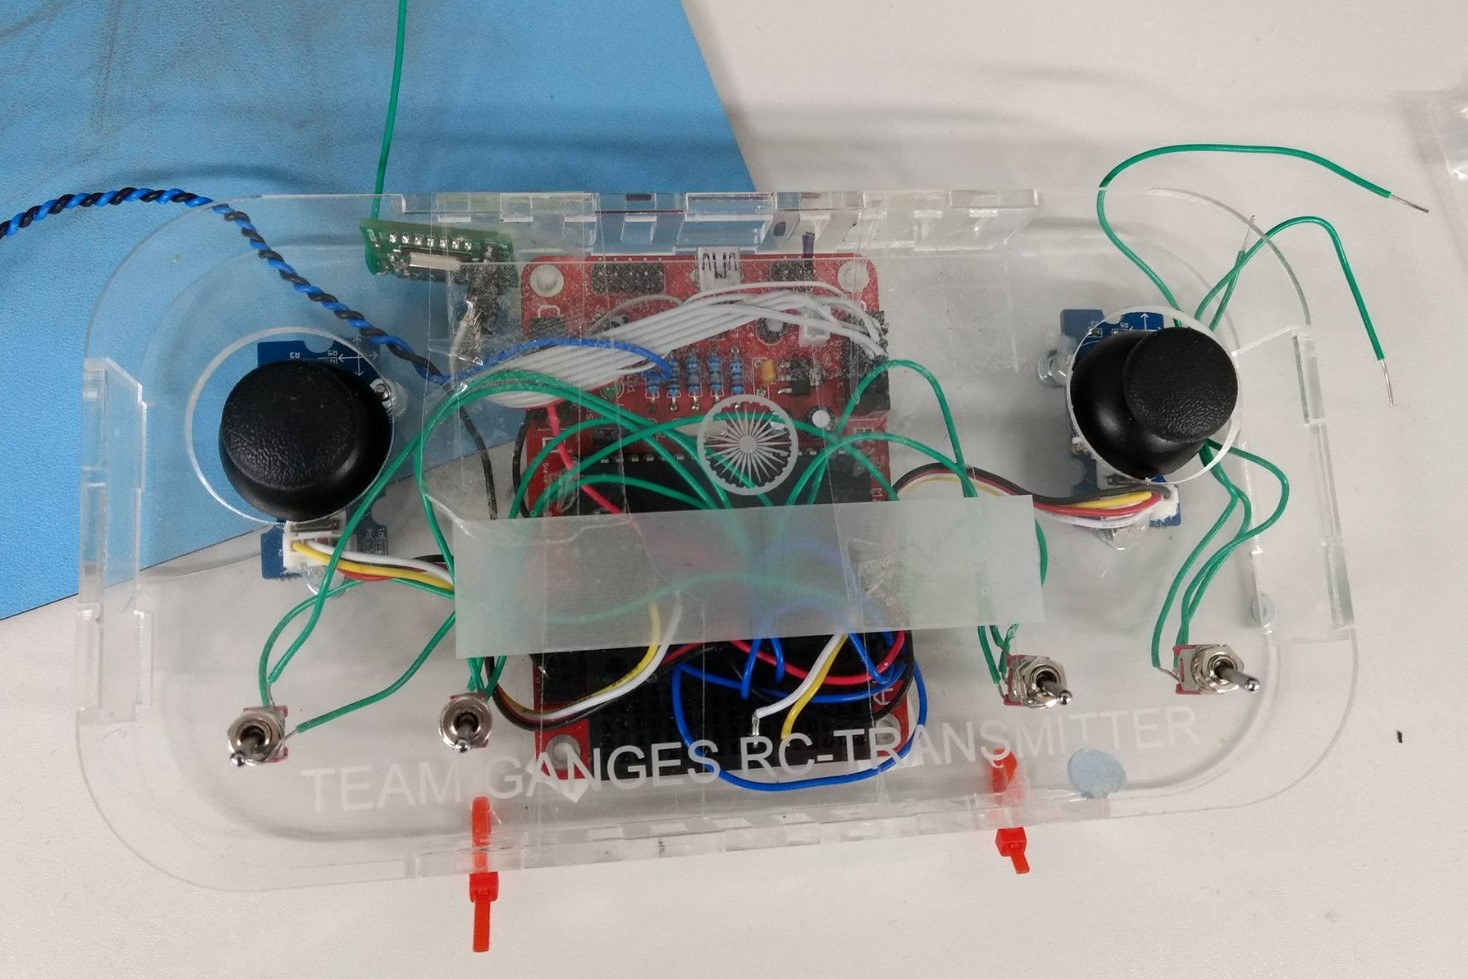
\includegraphics[width=0.9\linewidth]{remote.jpg} 
    \caption{Final build of the Pilot-Drone interface. Controller electronics inside an acrylic casing.}
    \label{fig:subim1}
    \end{subfigure}
    \begin{subfigure}{\textwidth}
    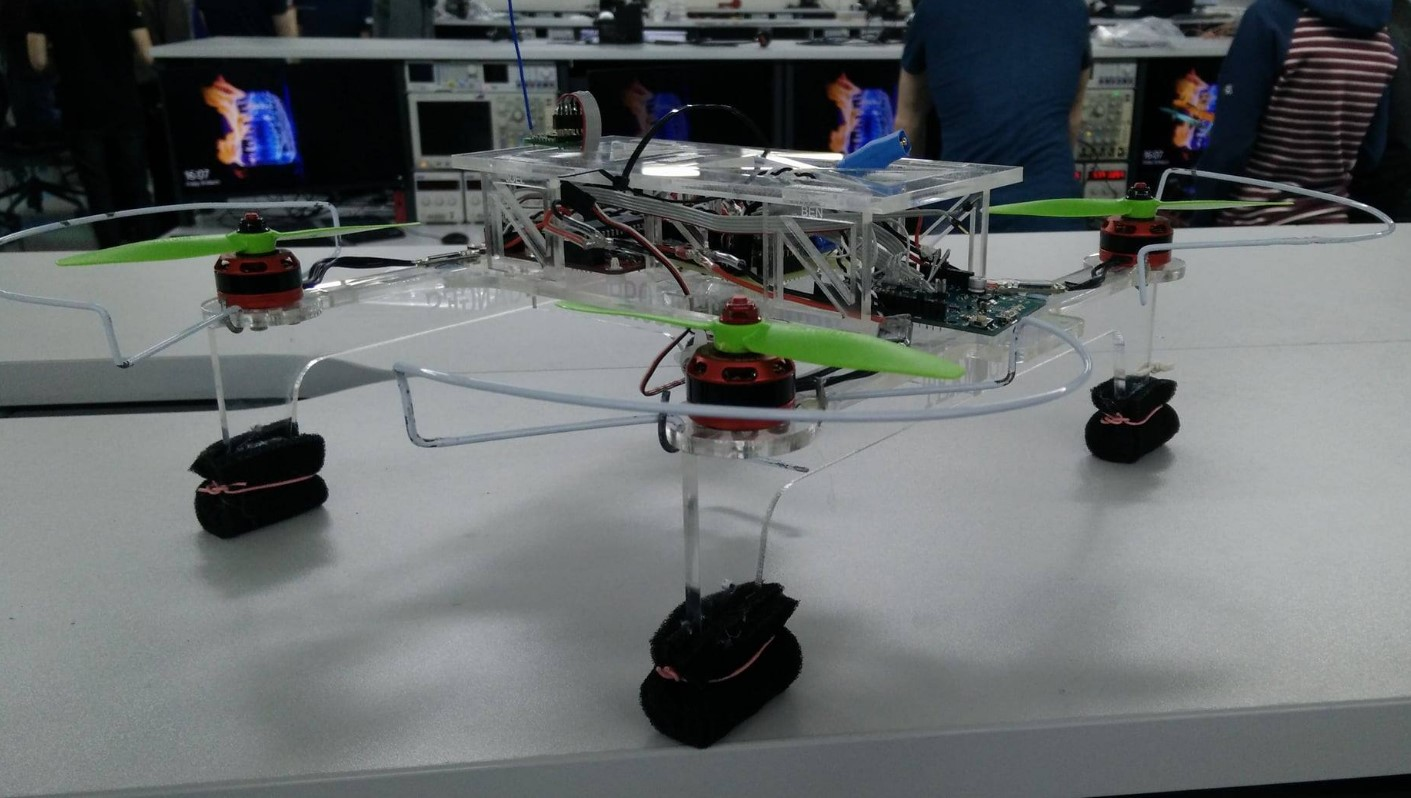
\includegraphics[width=0.9\linewidth]{drone.jpg}
    \caption{Final build of the Quad-copter UAV consisting of our communications and control systems, placed inside our chassis.}
    \label{fig:subim2}
    \end{subfigure}
    
    \label{fig:my_label}
\end{figure}
  
\end{document}